
%
%  $Description: Author guidelines and sample document in LaTeX 2.09$ 
%
%  $Author: ienne $
%  $Date: 1995/09/15 15:20:59 $
%  $Revision: 1.4 $
%

\documentclass[times, 10pt,twocolumn]{article} 
\usepackage{latex8}
\usepackage{times}
\usepackage[utf8]{inputenc}
\usepackage[brazil]{babel}
\usepackage{graphicx, url}
\usepackage{listings}

\usepackage[center]{caption}
\usepackage[alf,abnt-emphasize=bf,abnt-full-initials=yes]{abntcite} %Pacote abntex -  http://abntex.codigolivre.org.br/

%\documentstyle[times,art10,twocolumn,latex8]{article}

\usepackage[usenames]{color}

\definecolor{red}{rgb}{0.6,0,0} % for strings
\definecolor{green}{rgb}{0.25,0.5,0.35} % comments
\definecolor{purple}{rgb}{0.5,0,0.35} % keywords
\definecolor{docblue}{rgb}{0.25,0.35,0.75} % javadoc

\definecolor{DarkBlue}{rgb}{0,0,0.61}
\definecolor{DarkGreen}{rgb}{0,0.4,0}

\lstset{
  language=vhdl,
  basicstyle=\ttfamily\fontsize{10}{11}\selectfont,
  keywordstyle=\color{purple}\bfseries,
  stringstyle=\color{red},
  commentstyle=\color{green},
  morecomment=[s][\color{docblue}]{/*}{*/},
  numbers=left,
  numberstyle=\tiny\color{black},
  stepnumber=1,
  numbersep=10pt,
  tabsize=4,
  showspaces=false,
  showstringspaces=false,
  otherkeywords={\#include, \#define, \#pragma, \#typedef, dim3},
  emph={ __device__, __global__, __shared__, __host__, __constant__},
  emphstyle=\color{DarkBlue}\bfseries,
  emph={[2] printf, scanf},
  emphstyle=[2]\color{DarkGreen},
  extendedchars=true,
  frame=tb,
  breaklines=true
}

\usepackage{caption}
\DeclareCaptionFont{black}{\color{black}}

\renewcommand{\lstlistingname}{Código}

\usepackage{footnote}

%------------------------------------------------------------------------- 
% take the % away on next line to produce the final camera-ready version 
\pagestyle{empty}

%------------------------------------------------------------------------- 
\begin{document}
\begin{savenotes}
\title{Título do Artigo\footnote{Trabalho desenvolvido para a disciplina de BCC33B – Arquitetura e Organização de Computadores.}}


\author{Primeiro Autor1, Segundo Autor\\
Coordenação do Curso de Bacharelado em Ciência da Computação - COCIC\\
Universidade Tecnológica Federal do Paraná - UTFPR\\ 
Campus Campo Mourão\\
Campo Mourão, Paraná, Brasil\\
primeiro@email.com.br e segundo@email.com.br\\
% For a paper whose authors are all at the same institution, 
% omit the following lines up until the closing ``}''.
% Additional authors and addresses can be added with ``\and'', 
% just like the second author.
}

\maketitle
\thispagestyle{empty}

\begin{abstract}
   Apresente um resumo sobre o seu trabalho, lembre-se que o resumo deve introduzir, apresentar a idéia do seu trabalho de forma suficiente. O resumo de representar o seu trabalho, de maneira que ao ser impresso sozinho permita o leitor saber exatamente do que o trabalho trata. E caso lhe interesse o leitor irá ler o restante do conteúdo, as seções buscando a profundidade no tema.
   Blá Blá blá blá blá Blá Blá blá blá blá Blá Blá blá blá blá Blá Blá blá blá blá Blá Blá blá blá blá Blá Blá blá blá blá Blá Blá blá blá blá Blá Blá blá blá blá Blá Blá blá blá blá Blá Blá blá blá blá. Blá Blá blá blá blá Blá Blá blá blá blá Blá Blá blá blá blá Blá Blá blá blá blá Blá Blá blá blá blá Blá Blá blá blá blá Blá Blá blá blá blá Blá Blá blá blá blá Blá Blá blá blá blá Blá Blá blá blá blá, Blá Blá blá blá blá Blá Blá blá blá blá Blá Blá blá blá blá Blá Blá blá blá blá Blá Blá blá blá blá Blá Blá blá blá blá Blá Blá blá blá blá Blá Blá blá blá blá Blá Blá blá blá blá Blá Blá blá blá blá Blá Blá blá blá blá Blá Blá blá blá blá Blá Blá blá blá blá Blá Blá blá blá blá Blá Blá blá blá blá Blá Blá blá blá blá Blá Blá blá blá blá Blá Blá blá blá blá Blá Blá blá blá blá Blá Blá blá blá blá.
\end{abstract}
%------------------------------------------------------------------------- 
\section{Introdução} \label{sec_introducao}

A introdução como o nome diz, deve introduzir o leitor no contexto do trabalho, se for o caso, no problema que está sendo tratado, na solução proposta, nos resultados de experimentos. A introdução é um segundo nível de profundidade nos detalhes do trabalho. Um introdução bem escrita deve ser capaz de representar o trabalho, em seu nível de profundidade. É interessante também que na introdução sejam apresentadas as seções/partes do trabalho, como por exemplo,  “O presente artigo está organizado da seguinte forma. A próxima seção descreve sobre .... A seção 3 aborda tal assunto. Tais coisas relacionados aparecem na seção 4. A seção 5 explica bla bla bla. Os experimentos e as conclusões são mostrados nas seções 6 e 7. No final tem-se as referências utilizadas.”. Lembre-se esse é apenas um modelo.

%-------------------------------------------------------------------------
% Salva as notas de rodapé na primeira página.
\end{savenotes}

%------------------------------------------------------------------------- 
\section{Tópico do Texto} \label{sec_topico_texto}
Os tópicos do texto, devem possuir nomes significativos que tenham relação com o texto, no seu texto podem haver referências a outros trabalhos e artigos que foram consultados, estudados para a elaboração do trabalho. Referências devem ter o seguinte formato: [número], por exemplo \cite{Codishetal2000} refere-se ao primeiro trabalho apresentado na seção “Referências” e assim por diante no decorrer do texto.
As figuras devem ser referenciadas no seu texto e apresentadas conforme o modelo. Por exemplo, a Figura~{\ref{fig:figura-001}} apresenta como é feito o uso dos bancos da cache pelas tarefas.

\begin{figure}[!htb]
    \centering
    
\includegraphics{figuras/droopy.jpg}
    \caption{Legenda}
    \label{fig:figura-001}
\end{figure}

\section{Tópico do Texto 2} \label{sec_topico_texto_2}

As tabelas também devem ser referenciadas no texto. Por exemplo, tal e tal coisa estão presentes na Tabela~{\ref{tab:tabela-001}}. As tabelas podem ter o formato necessário para a apresentação dos valores, dados necessários à complementação do texto.


\begin{table}[h]
\caption {Sample Data}
\begin{center}
\begin{tabular}{|c|c|c|} \hline
$x$ & $y$ & $teste$  \\
\hline \hline
100 & 1 & Oi \\
\hline
85 & 2 & Sou  \\
\hline
70 & 4 & a  \\
\hline
50 & 8 & terceira  \\
\hline
36 & 15 & coluna  \\
\hline
20 & 25 & 0  \\
\hline
10 & 45 & 0  \\
\hline
\end{tabular}
\end{center}
\label{tab:tabela-001}
\end{table}


\subsection{Gráficos}
Gráficos também podem ser utilizados, nas mais diversas formas que os autores julgarem necessárias para demonstrar, provar ou simplesmente apresentar os resultados, estatísticas, enfim, qualquer informação que seja importante para complementar e apresentar visualmente ao leitor informações relevantes que complementem, agreguem informações ao texto escrito. Exemplo, na Figura~{\ref{fig:figura-002}} são apresentados os valores de consumo dinâmico no modo de execução SMT-16.

\begin{figure}[*H]
    \centering
    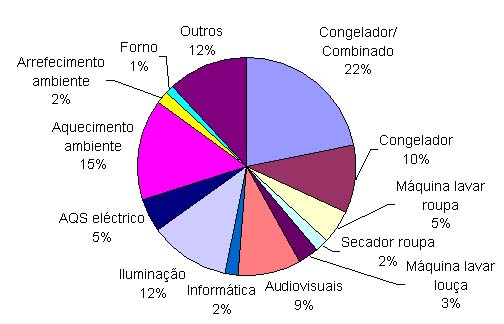
\includegraphics[width=.5\textwidth]{figuras/consumo.jpg}
    \caption{Consumo de Energia}
    \label{fig:figura-002}
\end{figure}

\subsection{Código fonte}

Código fonte pode ser inserido diretamente, conforme o exemplo no Código~{\ref{cod:codigo-direto}}.

\begin{lstlisting}[label=cod:codigo-direto,caption=Descrição VHDL de uma Porta AND de duas entradas.]
-- Project generated by script.
-- Date: Ter,06/11/2012-09:40:15
-- Author: a1061852
-- Comments: Entity Description: and2.
 
library ieee;
use ieee.std_logic_1164.all;
use ieee.std_logic_unsigned.all;
 
entity and2 is
port (A, B: in std_logic; C: out std_logic);
end and2;
 
architecture logica of and2 is
begin
  -- Commands.
  C <= A and B;
end logica;
\end{lstlisting}

Ou pode ser inserido de um arquivo, conforme no Código~{\ref{cod:codigo-arquivo}}.

\lstinputlisting[label=cod:codigo-arquivo,caption=Porta Ou Exclusivo ]{codigo/xor2.vhd}

A Figura~{\ref{fig:figura-003}}, apresenta um outro tipo de gráfico que pode ser utilizado, com já foi dito, qualquer tipo de gráfico pode ser utilizado para permitir ao leitor uma visualização de informações importantes.
Blá Blá blá blá blá Blá Blá blá blá blá Blá Blá blá blá blá Blá Blá blá blá blá Blá Blá blá blá blá Blá Blá blá blá blá Blá Blá blá blá blá Blá Blá blá blá blá Blá Blá blá blá blá Blá Blá blá blá blá.

Blá Blá blá blá blá Blá Blá blá blá blá Blá Blá blá blá blá Blá Blá blá blá blá Blá Blá blá blá blá Blá Blá blá blá blá Blá Blá blá blá blá Blá Blá blá blá blá Blá Blá blá blá blá Blá Blá blá blá blá

\begin{figure}[*H]
    \centering
    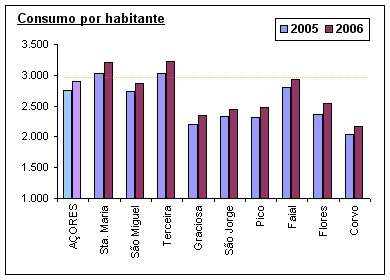
\includegraphics[width=.5\textwidth]{figuras/consumo-2.jpg}
    \caption{Consumo de Energia 2}
    \label{fig:figura-003}
\end{figure}

Blá Blá blá blá blá Blá Blá blá blá blá Blá Blá blá blá blá Blá Blá blá blá blá Blá Blá blá blá blá Blá Blá blá blá blá Blá Blá blá blá blá Blá Blá blá blá blá Blá Blá blá blá blá Blá Blá blá blá blá
Blá Blá blá blá blá Blá Blá blá blá blá Blá Blá blá blá blá Blá Blá blá blá blá Blá Blá blá blá blá Blá Blá blá blá blá Blá Blá blá blá blá Blá Blá blá blá blá Blá Blá blá blá blá Blá Blá blá blá blá.

\section{Blá Blá}
Blá Blá blá blá blá Blá Blá blá blá blá Blá Blá blá blá blá Blá Blá blá blá blá Blá Blá blá blá blá Blá Blá blá blá blá Blá Blá blá blá blá Blá Blá blá blá blá Blá Blá blá blá blá Blá Blá blá blá blá
Blá Blá blá blá blá Blá Blá blá blá blá Blá Blá blá blá blá Blá Blá blá blá blá Blá Blá blá blá blá Blá Blá blá blá blá Blá Blá blá blá blá Blá Blá blá blá blá Blá Blá blá blá blá Blá Blá blá blá blá
Blá Blá blá blá blá Blá Blá blá blá blá Blá Blá blá blá blá Blá Blá blá blá blá Blá Blá blá blá blá Blá Blá blá blá blá Blá Blá blá blá blá Blá Blá blá blá blá Blá Blá blá blá blá Blá Blá blá blá blá
Blá Blá blá blá blá Blá Blá blá blá blá Blá Blá blá blá blá Blá Blá blá blá blá Blá Blá blá blá blá Blá Blá blá blá blá Blá Blá blá blá blá Blá Blá blá blá blá Blá Blá blá blá blá Blá Blá blá blá blá
Blá Blá blá blá blá Blá Blá blá blá blá Blá Blá blá blá blá Blá Blá blá blá blá Blá Blá blá blá blá Blá Blá blá blá blá Blá Blá blá blá blá Blá Blá blá blá blá Blá Blá blá blá blá Blá Blá blá blá blá. 
Blá Blá blá blá blá Blá Blá blá blá blá Blá Blá blá blá blá Blá Blá blá blá blá Blá Blá blá blá blá Blá Blá blá blá blá Blá Blá blá blá blá Blá Blá blá blá blá Blá Blá blá blá blá Blá Blá blá blá blá
Blá Blá blá blá blá Blá Blá blá blá blá Blá Blá blá blá blá Blá Blá blá blá blá Blá Blá blá blá blá Blá Blá blá blá blá Blá Blá blá blá blá Blá Blá blá blá blá Blá Blá blá blá blá Blá Blá blá blá blá
Blá Blá blá blá blá Blá Blá blá blá blá Blá Blá blá blá blá Blá Blá blá blá blá Blá Blá blá blá blá Blá Blá blá blá blá Blá Blá blá blá blá Blá Blá blá blá blá Blá Blá blá blá blá Blá Blá blá blá bláBlá Blá blá blá blá Blá Blá blá blá blá Blá Blá blá blá blá Blá Blá blá blá blá Blá Blá blá blá blá Blá Blá blá blá blá Blá Blá blá blá blá Blá Blá blá blá blá Blá Blá blá blá blá Blá Blá blá blá blá.

\section{Conclusão}

Conclua as ideias, responda a questionamentos, discuta resultados obtidos e etc.
Os trabalhos utilizados para a elaboração do seu trabalho deve ser citado na seção “Referências” e referenciado no meio do texto, onde estiver as ideias associadas a ele. Lembre-se, copiar texto da Internet ou de qualquer outro trabalho e dizer que é de sua autoria é crime de Plágio. A utilização de textos oriundos da Internet pode ocorrer, mas com a devida cautela, pois a internet é um meio de livre publicação, não se tem a garantia da veracidade das informações publicadas. Sempre procure referenciar artigos científicos, livros, enfim, fontes mais seguras que uma página qualquer de internet.
Blá Blá blá blá blá Blá Blá blá blá blá Blá Blá blá blá blá Blá Blá blá blá blá Blá Blá blá blá blá Blá Blá blá blá blá Blá Blá blá blá blá Blá Blá blá blá blá Blá Blá blá blá blá Blá Blá blá blá blá
Blá Blá blá blá blá Blá Blá blá blá blá Blá Blá blá blá blá Blá Blá blá blá blá Blá Blá blá blá blá Blá Blá blá blá blá Blá Blá blá blá blá Blá Blá blá blá blá Blá Blá blá blá blá Blá Blá blá blá blá
Blá Blá blá blá blá Blá Blá blá blá blá Blá Blá blá blá blá Blá Blá blá blá blá Blá Blá blá blá blá Blá Blá blá blá blá Blá Blá blá blá blá Blá Blá blá blá blá Blá Blá blá blá blá Blá Blá blá blá blá
Blá Blá blá blá blá Blá Blá blá blá blá Blá Blá blá blá blá Blá Blá blá blá blá Blá Blá blá blá blá Blá Blá blá blá blá Blá Blá blá blá blá Blá Blá blá blá blá Blá Blá blá blá blá Blá Blá blá blá blá
Blá Blá blá blá blá Blá Blá blá blá blá Blá Blá blá blá blá Blá Blá blá blá blá Blá Blá blá blá blá Blá Blá blá blá blá Blá Blá blá blá blá Blá Blá blá blá blá Blá Blá blá blá blá Blá Blá blá blá blá. 
Blá Blá blá blá blá Blá Blá blá blá blá Blá Blá blá blá.

%------------------------------------------------------------------------- 
\nocite{ex1,ex2}
\bibliographystyle{latex8}
\bibliography{bibliografia}

\end{document}
